\documentclass[11pt,a4j]{jsarticle}
\title{アナログ回路Ⅱ}
\author{1413176 三村幸祐}
\date{2016/11/09 \, 2016/11/16}
\usepackage{booktabs}
\usepackage[dvipdfmx,hiresbb]{graphicx}
%\pagestyle{empty}

\begin{document}
  
 \tableofcontents \newpage
  
 \section{目的}
 アナログ回路に我々が期待する機能とは、様々な演算機能を持っており、それらを回路に委託すれば答えが帰ってくることである。
 
  その一例として、現在までに私たちは線形信号処理のアナログ回路について学んできた。これにより和、差、乗算、周波数フィルタリング、微分積分などを回路上で表現することが可能となった。
  
  しかし、その他の非線形の演算を行う場合これらの知識では足りない。それを補うのが今回の実験の目的であり、リミッタ回路による出力のデジタル表現、ヒステリシスコンパレータによる可逆性の入出力循環変化、絶対値回路による閾値付近の性質変化による線形の折れ曲がり、などによって主に入出力特性が折れ線で表現される非線形信号処理について理解する。
  
  %レベルシフタ
 \section{レベルシフタ}
  \subsection{原理}[1]
   
   今回使用するレベルシフタの回路を図\ref{fig:levelshifter}に、また理想的なレベルシフタで実現される原理グラフを図\ref{fig:risou_levelshifter}に示す。
   
   またこの理想的なレベルシフタの$V_i$に対する$V_o$の挙動は以下の式で表すことが出来る。
   \begin{equation}
   V_o = \frac{5}{3} V_i - 10 \label{equ:1}
   \end{equation}
   
   \begin{figure}[htbp]
  \centering
  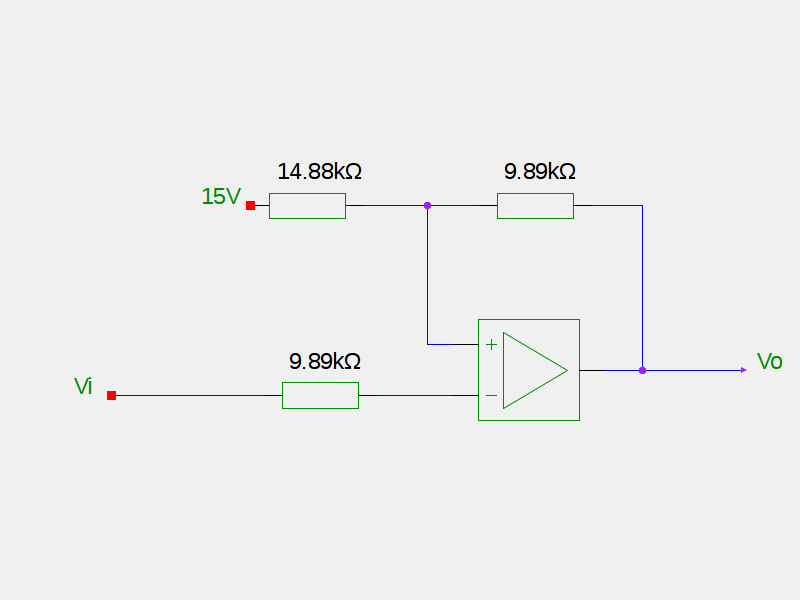
\includegraphics[width=8cm,clip]{levelshifter.png}
  \caption{レベルシフタの設計回路}
  \label{fig:levelshifter}
 \end{figure}%
   
   \begin{figure}[htbp]
  \centering
  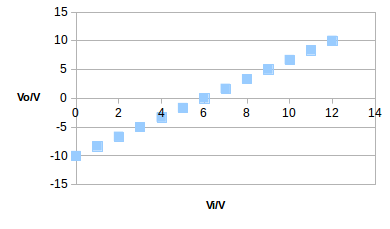
\includegraphics[width=8cm,clip]{risou_levelshifter.png}
  \caption{理想的なレベルシフタの原理グラフ}
  \label{fig:risou_levelshifter}
 \end{figure}
   
  \subsection{測定手順}
   ここでは、以降の実験で正電源から正負の入力を得る入力変換装置として用いるレベルシフタ回路を設計し、その挙動を検証。
   \begin{enumerate}
   \item 図\ref{fig:levelshifter}の回路を設計。
   \item 回路中の$V_i$に0~12Vの電圧を加え、その出力$V_o$の挙動を計測。
   \end{enumerate}
   
   
  \subsection{結果と考察} \label{sec:le_kousatu}
  レベルシフタの動作結果を図\ref{fig:1_0}に示した。この図を見ると、0~12Vの正の入力に対して、-10~10Vの一定の幅を持った正負の出力範囲が得られていることが分かる。したがってこれはレベルシフタとしての動作を反映していることを示し、さらに入力電圧に対して線形関数的に出力電圧が得られるため、以降実験の入力としてこの出力電圧を扱うに当たって、レベルシフタは非常に実験者からみても安定的で有効な回路である、ということが分かった。
  
  また、理想的なレベルシフタの原理グラフと比較してみても、測定グラフの原理グラフとの乖離はなく、実際測定グラフは式\ref{equ:1}の入出力挙動を、つまり入力が0~12Vに対して線形敵に出力が-10~10Vの間で変化している。
  
   \begin{figure}[htbp]
  \centering
  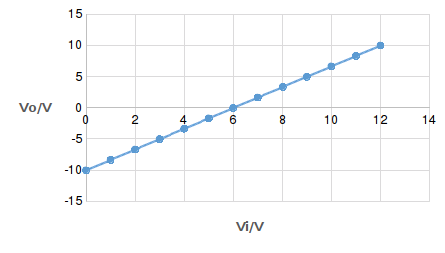
\includegraphics[width=8cm,clip]{1_0.png}
  \caption{レベルシフタの測定測定}
  \label{fig:1_0}
 \end{figure}%
   
   ところで今回扱ったレベルシフタは非反転型と呼ばれるものであるが、ここで反転型のレベルシフタについても少し述べておく。
   
   図\ref{fig:reverse}に反転型レベルシフタの回路図を示す。この回路図で本実験の非反転型レベルシフタと同範囲の出力を表現する場合には
   \begin{equation}
   V_o = -\frac{5}{3} V_i + 10
   \end{equation}
   となる設計を行う必要がある。
   
   すなわち図中の$R_{t4}$と$V_X$の値を考えると、
   \begin{eqnarray}
   V_i - V_X &=& 12I \nonumber \\
   V_i - V_o &=& 32I \nonumber
   \end{eqnarray}
   より、
   \begin{eqnarray}
   12(V_i - V_o) &=& 32 (V_i - V_X) \nonumber \\
   V_o &=& -\frac{5}{3} V_i + \frac{8}{3} V_X \nonumber
   \end{eqnarray}
   となる。よって、
   \begin{eqnarray}
   \frac{8}{3} V_X &=& 10 \nonumber \\
   V_X &=& 3.75 \verb|V| \nonumber
   \end{eqnarray}
   であり、ゆえに$R_{t3}$は次のようになる。
   \begin{eqnarray}
   V_X - 0 &=& 15 * \frac{12}{R_{t3} +12} \nonumber \\
   R_{t3} &=& 36 \verb|k| \Omega \nonumber
   \end{eqnarray}
   
   \begin{figure}[htbp]
  \centering
  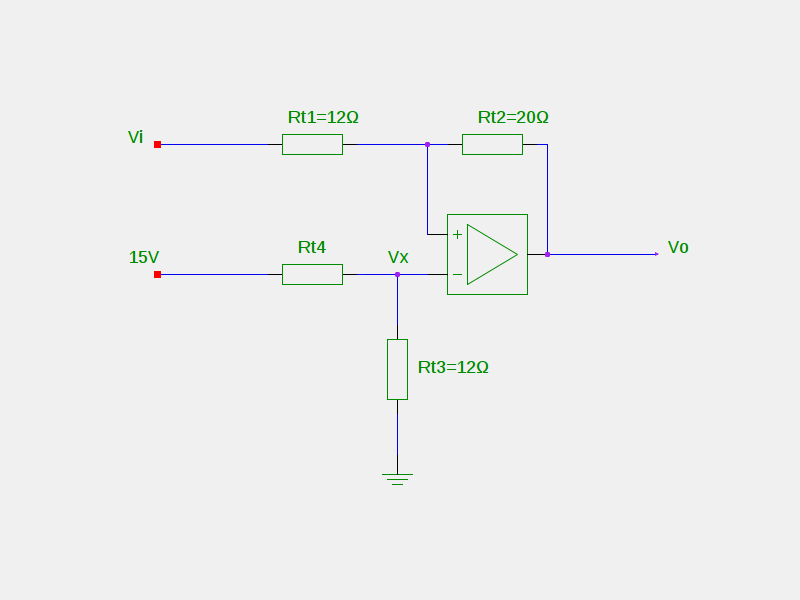
\includegraphics[width=8cm,clip]{reverse_levelshifter.png}
  \caption{反転型レベルシフタ}
  \label{fig:reverse}
 \end{figure}
   
   \clearpage
   
   %リミッタ
 \section{リミッタ}
  \subsection{オペアンプを用いないリミッタの入出力特性}
   \subsubsection{原理}[1]
    
    図\ref{fig:noamp_tokusei}にオペアンプを用いないリミッタ回路を示す。ただし、ここで各抵抗の値を
    \begin{itemize}
    \item $R_{S1}$=14.88k$\Omega$
    \item $R_{S2}$= 9.89k$\Omega$
    \item $R_{P}$=9.89k$\Omega$
    \item $R_{1}$=10.14k$\Omega$
    \end{itemize}
    としている。
    
    
    原理的に理想的なリミッタ回路は以下の2点の特性を示す。
    \begin{itemize}
    \item $V_i > 0$の時、$V_o = V_i$ V。
    \item $V_i < 0$の時、$V_o = 0$ V。
    \item 周波数依存性がない。
    \end{itemize}
    したがって理想的なリミッタの挙動は図\ref{fig:risou_limitter}に示すような形をとり、またそのグラフは以下の式で表される。
    
    \begin{eqnarray}
    V_o &=& V_o (V_i >0) \\
            &=& 0 (V_i < 0)
    \end{eqnarray}
    
    
    
    \begin{figure}[htbp]
  \centering
  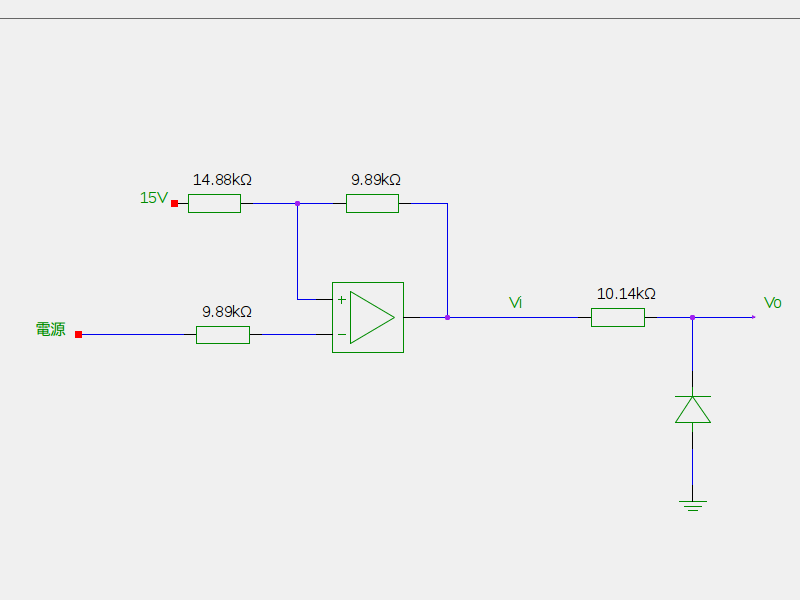
\includegraphics[width=8cm,clip]{noamp_tokusei.png}
  \caption{オペアンプを用いないリミッタの測定回路}
  \label{fig:noamp_tokusei}
 \end{figure}%
    
    \begin{figure}[htbp]
  \centering
  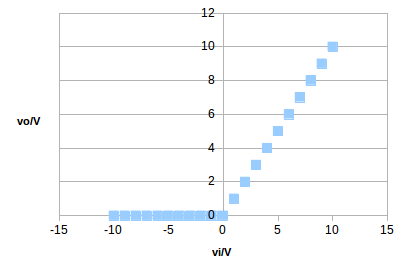
\includegraphics[width=8cm,clip]{risou_limitter.png}
  \caption{理想的なリミッタの原理グラフ}
  \label{fig:risou_limitter}
 \end{figure}
 
  また図\ref{fig:noamp_tokusei}のダイオードにかかる電圧$V_D$と電流$I_D$は、以下の換算式から求めることができる。このリミッタ特性からダイオード特性への換算式は以降、オペアンプを用いないリミッタ、及びオペアンプを用いたリミッタの考察において使用する。
  
  \begin{eqnarray}
  V_D &=& - V_o \label{equ:6} \\
  I_D &=& \frac{V_o - V_i}{R_1} \label{equ:7}
  \end{eqnarray}
    
    
    
   \subsubsection{測定手順}
    直流電源について、リミッタ回路を用いて整流作用の動作を確認。
    \begin{enumerate}
    \item 図\ref{fig:noamp_tokusei}を設計。
    \item レベルシフタによる変換後の入力$V_i$を(-4V~+4V)の範囲で変動させながら、出力$V_o$を測定。
    \end{enumerate}
    
   \subsubsection{結果と考察} \label{sec:noamp_tokusei}
    図\ref{fig:1_1_noamp_PS}にオペアンプを用いないリミッタの入出力特性を示す。
    この図を見ると、入力電圧が正の時は傾きが1の線形特性、入力電圧が負の時は0に近い一定の負の出力が得られることが分かる。リミッタ回路の特性上、入力が負の場合には回路上のダイオードに正のバイアスが、入力が正の場合にはダイオードに負のバイアスがかかる。つまりリミッタ回路の入出力特性は以下のようにまとめることができる。
    \begin{itemize}
    \item 入力電圧$V_i < 0$Vの時、出力電圧$V_o$は0V
    \item 入力電圧$V_i > 0$Vの時、出力電圧$V_o$=$V_i$
    \end{itemize}
    
    
    \begin{figure}[htbp]
  \centering
  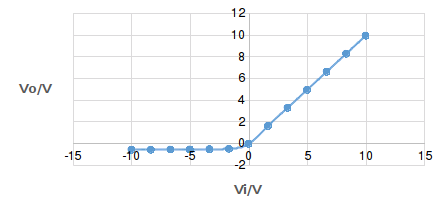
\includegraphics[width=8cm,clip]{1_1_noamp_PS.png}
  \caption{オペアンプを用いないリミッタの入出力特性}
  \label{fig:1_1_noamp_PS}
 \end{figure}%
    
    これでリミッタ回路の入出力特性を確認することができたわけだが、ダイオードをスイッチとして使用した例である。この図からは入力電圧が微小な負の値をもつ所から出力電圧が立ち上がり始めていることも確認できるため、ダイオードの立ち上がり電圧もデータに現れていることもわかる。
    
    また本実験の回路図中のダイオードの電流電圧特性を図\ref{fig:b_noamp}に示す。このグラフから今回使用したダイオードが、入力が負の時出力が0、また入力が0.5~0.7Vとなったときに出力が大きくなりだす、という一般的なシリコンダイオードの入出力特性を示していることが分かる。
    
    \begin{figure}[htbp]
  \centering
  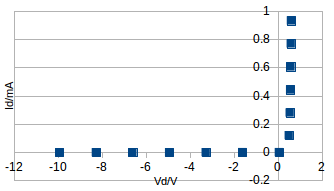
\includegraphics[width=8cm,clip]{b_noamp.png}
  \caption{オペアンプなしリミッタにおけるダイオードの電流電圧特性}
  \label{fig:b_noamp}
 \end{figure}
    
  \subsection{オペアンプを用いないリミッタの入出力波形観測}
   \subsubsection{原理}
    
    図\ref{fig:noamp_wave}にオペアンプを用いないリミッタの波形観測回路を示す。
    
    \begin{figure}[htbp]
  \centering
  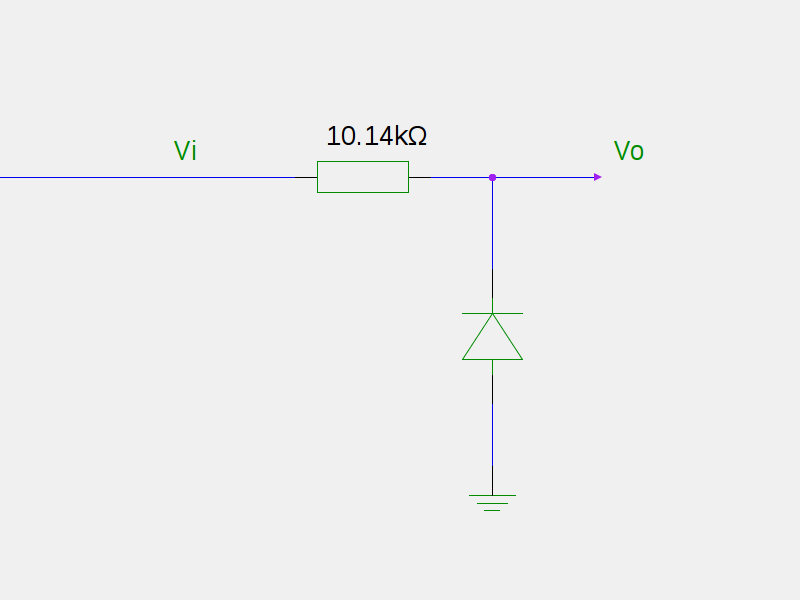
\includegraphics[width=8cm,clip]{noamp_wave.png}
  \caption{オペアンプを用いないリミッタの波形観測回路}
  \label{fig:noamp_wave}
 \end{figure}%
    
   \subsubsection{測定手順}
    交流電源について、リミッタ回路の整流作用を検証。
    \begin{enumerate}
    \item 図\ref{fig:noamp_wave}の回路を設計。
    \item 交流電源を波形(ex.正弦波、三角波)、振幅、周波数などによって変動させ、それぞれの入力に対してその出力波形を観測。
    \end{enumerate}
    
   \subsubsection{結果と考察} \label{sec:noamp_wave}
    
    オペアンプを用いないリミッタの入出力波形を、正弦波、入力周波数、電圧によって測定した3つのサンプルデータをそれぞれ図\ref{fig:noamp_f1V2}、図\ref{fig:noamp_sankaku}、図\ref{fig:noamp_f100V4}に示す。
    
    
    \begin{figure}[htbp]
  \centering
  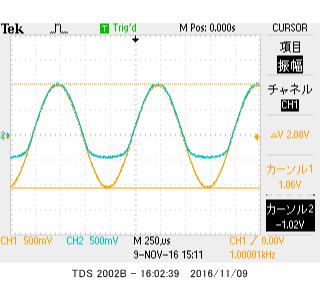
\includegraphics[width=8cm,clip]{1_1_noampFG_f1V2_ViVo.png}
  \caption{オペアンプを用いないリミッタの入出力波形(正弦波,入力周波数1kHz,電圧2Vpp)}
  \label{fig:noamp_f1V2}
 \end{figure}%
 
 \begin{figure}[htbp]
  \centering
  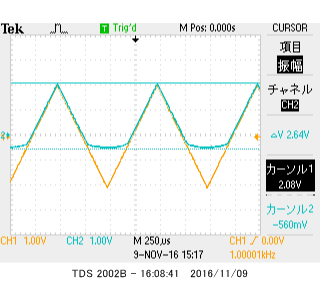
\includegraphics[width=8cm,clip]{1_1_noampFG_f1V4sankaku_ViVo.png}
  \caption{オペアンプを用いないリミッタの入出力波形(三角波,入力周波数1kHz,電圧4Vpp)}
  \label{fig:noamp_sankaku}
 \end{figure}%
 
 \begin{figure}[htbp]
  \centering
  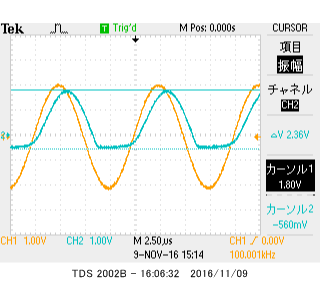
\includegraphics[width=8cm,clip]{1_1_noampFG_f100V4_ViVo.png}
  \caption{オペアンプを用いないリミッタの入出力波形(正弦波,入力周波数100kHz,電圧4Vpp)}
  \label{fig:noamp_f100V4}
 \end{figure}%
    
    入力周波数が1kHzの2つのデータを見てみると、入力が正の領域で入出力が1対1の関係になっている。負の方向に少し出力が浸透しているものダイオードの立ち上がり電圧による影響であろう。
    一方、入力周波数が100kHzのデータは振幅だけなら大きな変化はないものの、時間的な遅延が生じていることが確認できる。これはダイオードの含有する静電容量によるものだと考えられ、周波数が大きくなるとさらに大きな影響を及ぼすものだと予測できる。
    
    したがってここから、リミッタ回路は直流利用では問題なく利用できるが、交流として利用する際には、使用する周波数帯には気をつけなければならないということが分かった。
    
    最後にリミッタ回路を半波整流と見なしたときの平均電圧の計算を付録に掲載する。
    
    
  \subsection{オペアンプを用いたリミッタの入出力特性}
   \subsubsection{原理}
    
    図\ref{fig:amp_tokusei}にオペアンプを用いたリミッタ測定回路を示す。
    
    \begin{figure}[htbp]
  \centering
  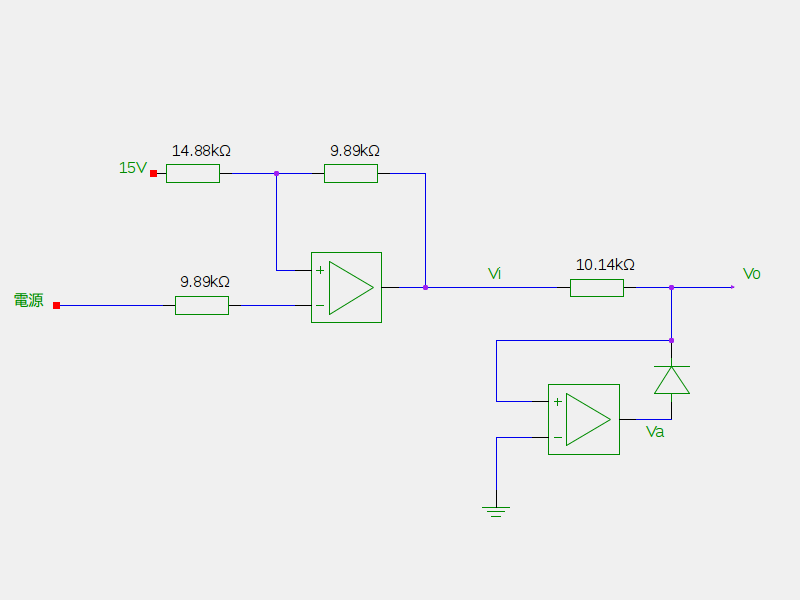
\includegraphics[width=8cm,clip]{amp_tokusei.png}
  \caption{オペアンプを用いたリミッタの測定回路}
  \label{fig:amp_tokusei}
 \end{figure}%
    
   \subsubsection{測定手順}
    オペアンプを用いたリミッタ回路について、直流電源に対する挙動を測定。
    \begin{enumerate}
    \item 図\ref{fig:amp_tokusei}の回路を設計。
    \item $V_i$を-4Vから+4Vまで変動させ、その出力を測定。
    \end{enumerate}
    
   \subsubsection{結果と考察} \label{sec:amp_tokusei}
    次の図\ref{fig:1_1_amp_PS_ViVo}、図\ref{fig:1_1_amp_PS_ViVa}にそれぞれ入力電圧に対するリミッタの出力、そしてオペアンプの出力電圧特性を示した。
    
    まず図\ref{fig:1_1_amp_PS_ViVo}をみてみる。このデータは定性的には先述のオペアンプを用いない場合の入出力特性と同様に見える。しかし今回の場合はマイナス側への出力電圧の浸透がなく、さらに立ち上がり部分の0に近づいている。
    
    さらに図\ref{fig:1_1_amp_PS_ViVa}を見ると、入力の0Vを境に離散的にオペアンプの出力は0Vから-14Vまで変わっている。このオペアンプの性質によって、オペアンプありのオペアンプなしとの違いは、
    \begin{itemize}
    \item リミット電圧のスイッチとしてのon,offへの切り替え性能の向上
    \item スイッチoff時の電圧漏れだしの防止
    \end{itemize}
    などが主にあげられる。
    
    また、式\ref{equ:6}、\ref{equ:7}によってリミッタの入出力特性から換算したダイオードの電流電圧特性を図\ref{fig:b_amp}に示す。この電流電圧特性は前述のリミッタ特性と同様に、オペアンプを用いない場合に比べてスイッチングのエッジが鋭くなっている。つまり、この仮想ダイオードの閾値が0V、かつ極めて小さな入力の変化で出力が大きくなっている。ここからオペアンプを用いることによる、ダイオードの入出力特性による順方向の閾値を負に増幅(小さくする)し、スイッチとしての機能を向上させていることがわかる。
    
    \begin{figure}[htbp]
  \centering
  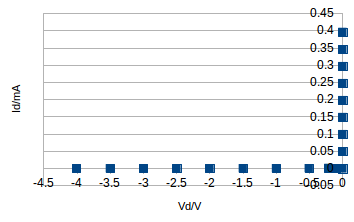
\includegraphics[width=8cm,clip]{b_amp.png}
  \caption{オペアンプありリミッタにおけるダイオードの入出力特性}
  \label{fig:b_amp}
 \end{figure}
    
    \begin{figure}[htbp]
  \centering
  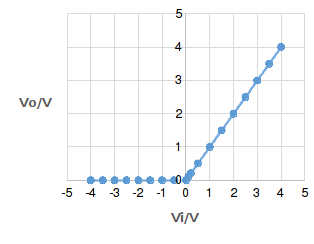
\includegraphics[width=8cm,clip]{1_1_amp_PS_ViVo.png}
  \caption{オペアンプを用いたリミッタの入出力特性}
  \label{fig:1_1_amp_PS_ViVo}
 \end{figure}%
   
   \begin{figure}[htbp]
  \centering
  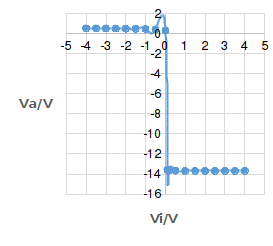
\includegraphics[width=8cm,clip]{1_1_amp_PS_ViVa.png}
  \caption{リミッタの入力電圧とオペアンプの出力電圧の特性}
  \label{fig:1_1_amp_PS_ViVa}
 \end{figure}%
    
    
  \subsection{オペアンプを用いたリミッタの入出力波形観測}
   \subsubsection{原理}
    
    図\ref{fig:amp_wave}にオペアンプを用いたリミッタの波形観測回路を示す。
    
    \begin{figure}[htbp]
  \centering
  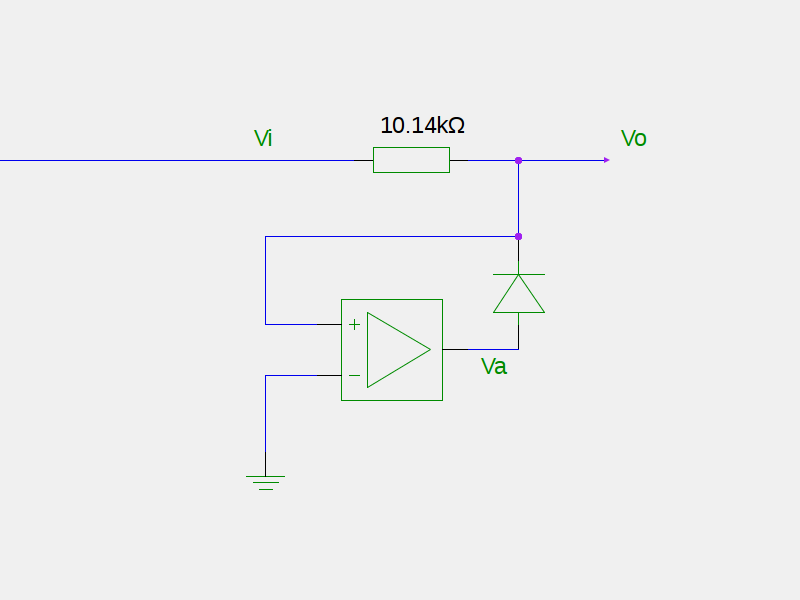
\includegraphics[width=8cm,clip]{amp_wave.png}
  \caption{オペアンプを用いたリミッタの波形観測回路}
  \label{fig:amp_wave}
 \end{figure}%
    
   \subsubsection{測定手順}
    オペアンプを用いたリミッタ回路について、交流電源に対する出力波形を観測。
    \begin{enumerate}
    \item 図\ref{fig:amp_wave}の回路を設計。
    \item 交流電源を波形(ex.正弦波、三角波)、振幅、周波数などによって変動させ、それぞれの入力に対してその出力波形を観測。
    \end{enumerate}
    
   \subsubsection{結果と考察} \label{sec:amp_wave}
    図\ref{fig:ampFGf1v2vivo},\ref{fig:ampFGf1v2viva}に正弦波で周波数1kHzの入力に対するデータを、図\ref{fig:ampFGf1v4vivo},\ref{fig:ampFGf1v4viva}に三角波で周波数1kHzの入力に対するデータを、そして最後の図\ref{fig:ampFGf100v4}に正弦波で周波数1kHzの入力に対するデータを示す。
    
    ここでも上述の入出力特性に関する特性と同様に、周波数が1kHzで低い状態ではその挙動はオペアンプなしと変わらない。
    
    ただし、高周波数、つまり100kHzになると振幅の減衰と位相の遅延が確認できる。理想的なリミッタでは遅延などはなく、入力値と出力値は1対1に対応しているはずである。
    
    ここで考えられるのはダイオードの空乏層容量による仮想的なコンデンサーである。このコンデンサーにより電子の伝送に遅延があり、またそのコンデンサーとしてのダイオードに電子が蓄積していくためにエネルギーの保存から出力側にかかる電圧値が小さくなっているものだといえる。[2]
    
    最後にリミッタ回路を半波整流と見なしたときの平均電圧の計算を付録に掲載する。
    
    \begin{figure}[htbp]
  \centering
  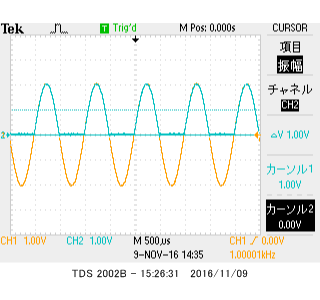
\includegraphics[width=8cm,clip]{1_1_ampFG_f1V2_ViVo.png}
  \caption{オペアンプを用いたリミッタの入出力波形(正弦波,入力周波数1kHz,電圧2Vpp)}
  \label{fig:ampFGf1v2vivo}
 \end{figure}%
 
 \begin{figure}[htbp]
  \centering
  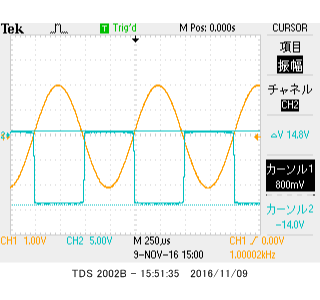
\includegraphics[width=8cm,clip]{1_1_ampFG_f1V2_ViVa.png}
  \caption{リミッタの入力電圧とオペアンプの出力電圧(正弦波,入力周波数1kHz,電圧2Vpp)}
  \label{fig:ampFGf1v2viva}
 \end{figure}%
 
 \begin{figure}[htbp]
  \centering
  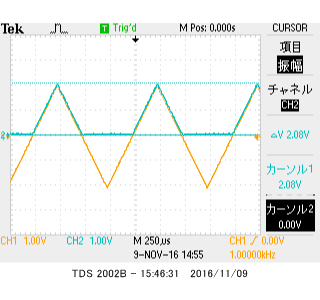
\includegraphics[width=8cm,clip]{1_1_ampFG_f1V4sankaku_ViVo.png}
  \caption{オペアンプを用いたリミッタの入出力波形(三角波,入力周波数1kHz,電圧4Vpp)}
  \label{fig:ampFGf1v4vivo}
 \end{figure}%
 
 \begin{figure}[htbp]
  \centering
  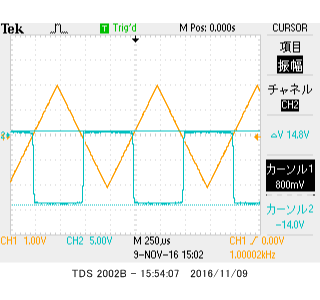
\includegraphics[width=8cm,clip]{1_1_ampFG_f1V4sankaku_ViVa.png}
  \caption{リミッタの入力電圧とオペアンプの出力電圧(三角波,入力周波数1kHz,電圧4Vpp)}
  \label{fig:ampFGf1v4viva}
 \end{figure}%
 
 \begin{figure}[htbp]
  \centering
  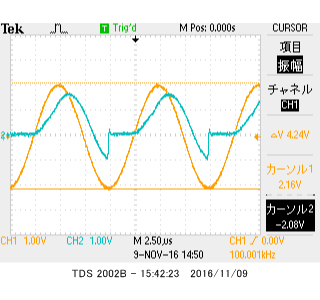
\includegraphics[width=8cm,clip]{1_1_ampFG_f100V4_ViVo.png}
  \caption{オペアンプを用いたリミッタの入出力波形(正弦波,入力周波数100kHz,電圧4Vpp)}
  \label{fig:ampFGf100v4}
 \end{figure}%
  
  
  \clearpage
    
  %ヒステリシスコンパレータ回路
 \section{ヒステリシスコンパレータ回路}
  \subsection{ヒステリシスコンパレータの入出力特性}
   \subsubsection{原理}[1]
    
    図\ref{fig:histeri_tokusei}にヒステリシスコンパレータの測定回路を、また理想的なヒステリシスコンパレータの原理グラフを図\ref{fig:risou_histeri}に示す。ただし図\ref{fig:risou_histeri}中に記している電圧値及び電流値は便宜上、仮に設定したものである。
    
    \begin{figure}[htbp]
  \centering
  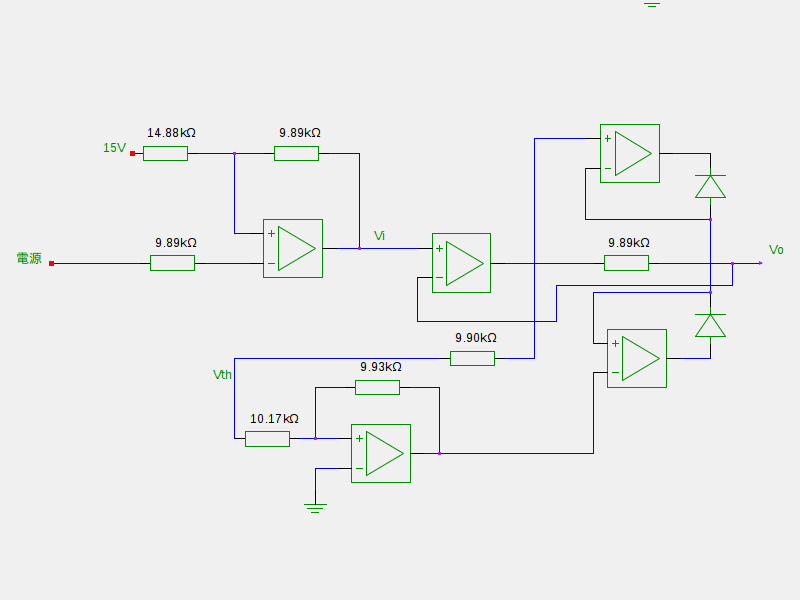
\includegraphics[width=8cm,clip]{histeri_tokusei.png}
  \caption{ヒステリシスコンパレータの測定回路}
  \label{fig:histeri_tokusei}
 \end{figure}%
    
    \begin{figure}[htbp]
  \centering
  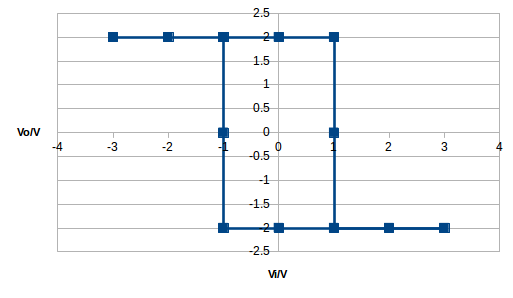
\includegraphics[width=8cm,clip]{risou_histeri.png}
  \caption{理想的なヒステリシスコンパレータの原理グラフ}
  \label{fig:risou_histeri}
 \end{figure}
    
   \subsubsection{測定手順}
    PS出力電圧$V_{th}$、コンパレータ入力電圧$V_i$に対する、ヒステリシスコンパレータの特性を測定。
    \begin{enumerate}
    \item 図\ref{fig:histeri_tokusei}の回路を設計。
    \item PS出力電圧$V_{th}$、コンパレータ入力電圧$V_i$を変動させ、コンパレータ出力$V_o$を測定。
    \end{enumerate}
    
   \subsubsection{結果と考察}
    PS出力電圧$V_{th}$を2V,1Vとして測定したヒステリシスのデータをそれぞれ図\ref{fig:1_2_histeri_Vth2},図\ref{fig:1_2_histeri_Vth1}に示す。
    
    \begin{figure}[htbp]
  \centering
  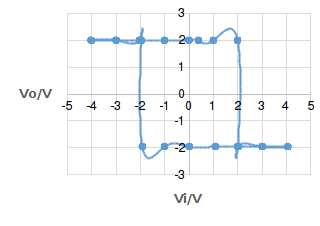
\includegraphics[width=8cm,clip]{1_2_histeri_Vth2.png}
  \caption{PS出力電圧$V_{th}$=2Vの時のヒステリシスコンパレータの入出力特性}
  \label{fig:1_2_histeri_Vth2}
 \end{figure}%
    
 \begin{figure}[htbp]
  \centering
  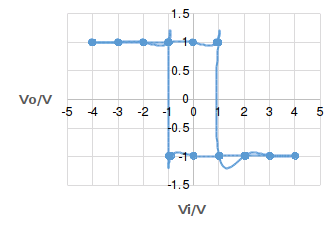
\includegraphics[width=8cm,clip]{1_2_histeri_Vth1.png}
  \caption{PS出力電圧$V_{th}$=1Vの時のヒステリシスコンパレータの入出力特性}
  \label{fig:1_2_histeri_Vth1}
 \end{figure}%
    
    
    
  \subsection{ヒステリシスコンパレータの入出力波形観測}
   \subsubsection{原理}
    
    図\ref{fig:histeri_wave}にヒステリシスコンパレータの波形観測回路を示す。
    
    \begin{figure}[htbp]
  \centering
  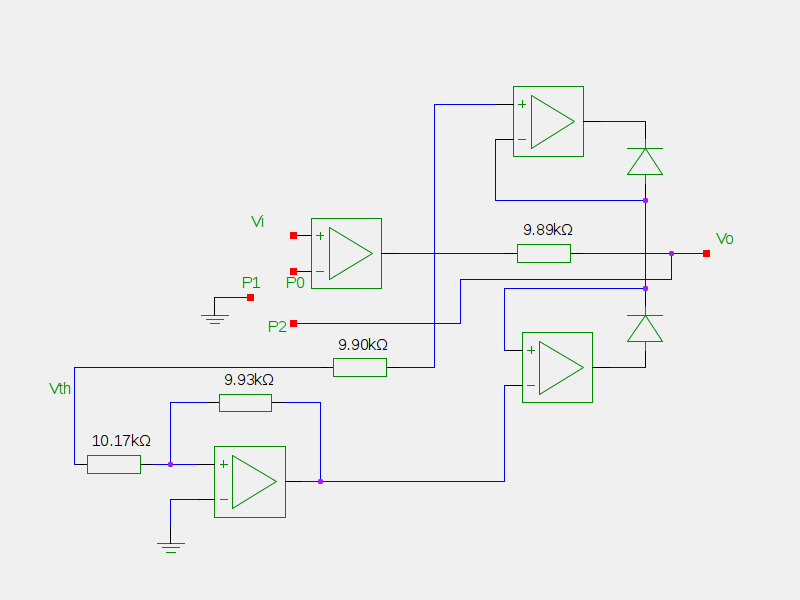
\includegraphics[width=8cm,clip]{histeri_wave.png}
  \caption{ヒステリシスコンパレータの波形観測回路}
  \label{fig:histeri_wave}
 \end{figure}%
    
   \subsubsection{測定手順}
    
    図\ref{fig:histeri_wave}の回路を設計。その後、以下の基本波形・模擬ノイズ波形観測について測定。
    
    基本波形について。
    \begin{enumerate}
    \item 図\ref{fig:histeri_wave}の$P_0$を$P_2$に接続。
    \item PS出力電圧$V_{th}$、波形(ex.正弦波、三角波)、周波数、振幅による波形の変動を観測。
    \end{enumerate}
    
    模擬ノイズ波形観測について。
    \begin{enumerate}
    \item 図\ref{fig:histeri_wave}の$P_0$を$P_2$に接続。
    \item 波形を模擬ノイズ重畳波形に設定。正弦波6V$_{pp}$(入力)+三角波1V$_{pp}$(ノイズ)、正弦波6V$_{pp}$(入力)+三角波4V$_{pp}$(ノイズ)について測定。
    \item 図\ref{fig:histeri_wave}の$P_0$を$P_1$に接続を変更。これによりヒステリシスから通常のコンパレータ回路となる。
    \item 通常コンパレータについて、2の操作を同様に行う。
    \end{enumerate}
    
   \subsubsection{結果と考察} \label{sec:histeri}
    
    図\ref{fig:histeri_2-1}~\ref{fig:histeri_1-1}には基本波形観測の波形データを、図\ref{fig:noise_before_6-1_big}~\ref{fig:noise_after_6-1_small}にはノイズ波形観測の波形データをそれぞれ示す。
    
    \begin{figure}[htbp]
  \centering
  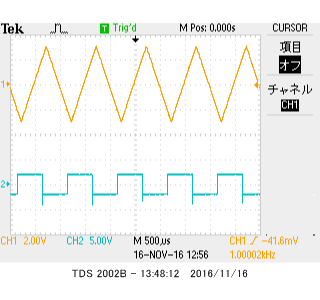
\includegraphics[width=8cm,clip]{1_2_histeri_Vth2f1V6sankaku_ViVo.png}
  \caption{ヒステリシスコンパレータの波形観測(三角波、PS=2V、振幅$V_{pp}$=6V、周波数1kHz)}
  \label{fig:histeri_2-1}
 \end{figure}
 
 \begin{figure}[htbp]
  \centering
  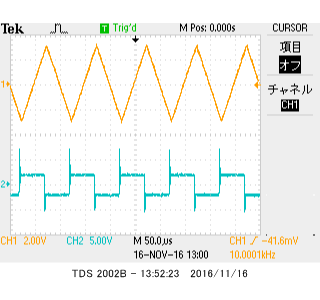
\includegraphics[width=8cm,clip]{1_2_histeri_Vth2f10V6sankaku_ViVo.png}
  \caption{ヒステリシスコンパレータの波形観測(三角波、PS=2V、振幅$V_{pp}$=6V、周波数10kHz)}
  \label{fig:histeri_2-10}
 \end{figure}
 
 \begin{figure}[htbp]
  \centering
  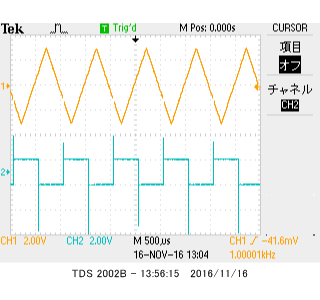
\includegraphics[width=8cm,clip]{1_2_histeri_Vth1f1V6sankaku_ViVo.png}
  \caption{ヒステリシスコンパレータの波形観測(三角波、PS=1V、振幅$V_{pp}$=6V、周波数1kHz)}
  \label{fig:histeri_1-1}
 \end{figure}
 	
 	まずのノイズのない波形を見る。理想的なヒステリシスコンパレータではその入出力特性から周期内の立ち上がり及び立ち下がりにおいて同程度の大きさの振れ幅で1周期振動して元の大きさに戻る。上記のPSが2Vの時の2つのデータはそのような挙動を示しているが、しかし、PSが1Vの時のデータでは負の方向により大きく振動していることが確認できる。これはPSと直結したオペアンプにかかる電圧が小さなPS電源と$R_4$によって小さくなり、その出力先のダイオードの空乏層容量によって正と負の出力に差が生じているのだと考えられる。
 	
 \begin{figure}[htbp]
  \centering
  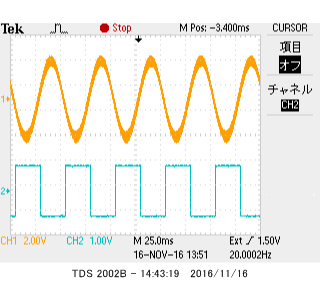
\includegraphics[width=8cm,clip]{1_2_noise_before_6-1_BigScale.png}
  \caption{ヒステリシスコンパレータの入力・ノイズ波形(正弦波6V$_{pp}$(入力)+三角波1V$_{pp}$(ノイズ))(縮小スケール)}
  \label{fig:noise_before_6-1_big}
 \end{figure}
 
 \begin{figure}[htbp]
  \centering
  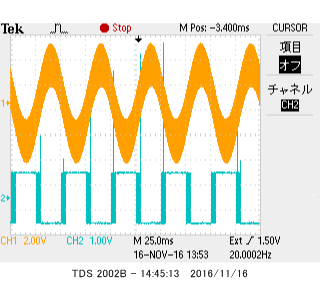
\includegraphics[width=8cm,clip]{1_2_noise_before_6-4_BigScale}
  \caption{ヒステリシスコンパレータの入力・ノイズ波形(正弦波6V$_{pp}$(入力)+三角波4V$_{pp}$(ノイズ))(縮小スケール)}
  \label{fig:noise_before_6-4_big}
 \end{figure}
 
 \begin{figure}[htbp]
  \centering
  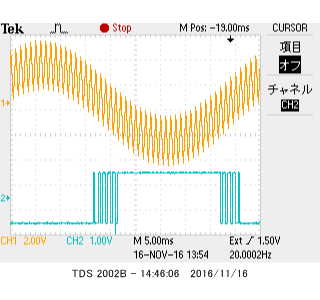
\includegraphics[width=8cm,clip]{1_2_noise_before_6-4_SmallScale.png}
  \caption{ヒステリシスコンパレータの入力・ノイズ波形(正弦波6V$_{pp}$(入力)+三角波4V$_{pp}$(ノイズ))(拡大スケール)}
  \label{fig:noise_before_6-4_small}
 \end{figure}
 
 \begin{figure}[htbp]
  \centering
  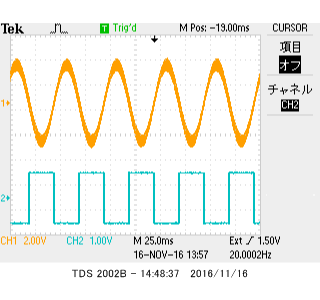
\includegraphics[width=8cm,clip]{1_2_noise_after_6-1_BigScale.png}
  \caption{通常コンパレータの入力・ノイズ波形(正弦波6V$_{pp}$(入力)+三角波1V$_{pp}$(ノイズ))(縮小スケール)}
  \label{fig:noise_after_6-1_big}
 \end{figure}
 
 \begin{figure}[htbp]
  \centering
  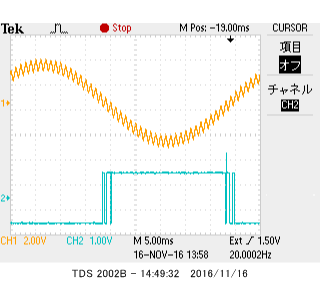
\includegraphics[width=8cm,clip]{1_2_noise_after_6-1_SmallScale.png}
  \caption{通常コンパレータの入力・ノイズ波形(正弦波6V$_{pp}$(入力)+三角波1V$_{pp}$(ノイズ))(拡大スケール)}
  \label{fig:noise_after_6-1_small}
 \end{figure}
    
    
    
    また、ヒステリシスコンパレータによるノイズが含まれている波形の閾値処理について考える。上記のノイズを含む波形観測のデータからヒステリシスコンパレータの方がその入力値が閾値を越えることによる出力のデジタル的な返歌を利用して低振幅のノイズを除去することができていることがわかる。つまりヒステリシスコンパレータの入力の閾値がそのコンパレータのヒステリシス幅と言えるが、ノイズ除去の性能はこのヒステリシス幅によっても変動する。ヒステリシスの幅より振幅の小さい信号が除去されることになるが、ここには利点と欠点が存在する。
    
    ヒステリシス幅を大きくする利点は、より振幅が大きくなったノイズも除去することができるという点である。閾値を大きくすることで除去できるノイズの最大振幅をあげることに由来している。
    
    一方、その幅を大きくする際の欠点は、意味のある信号も小さな振幅部分などだと意図せず除去してしまうという点。信号とノイズの区別をしているわけではないため、両者関係なく小さな信号は除去してしまう。
    
    したがってヒステリシス幅はただ大きくすれば良いということではなく、伝達したい信号の振幅の大きさと相互的に調節していかなくてはいけない。
    
    
    \clearpage
    
    %絶対値回路
 \section{絶対値回路}
  \subsection{絶対値回路の入出力特性}
   \subsubsection{原理}
    
    図\ref{fig:abs_tokusei}に絶対値回路の測定回路を、また基準電圧が0Vと1Vの理想的な絶対値回路の原理グラフを図\ref{fig:risou_absr0}、\ref{fig:risou_absr1}に示す。
    
    \begin{figure}[htbp]
  \centering
  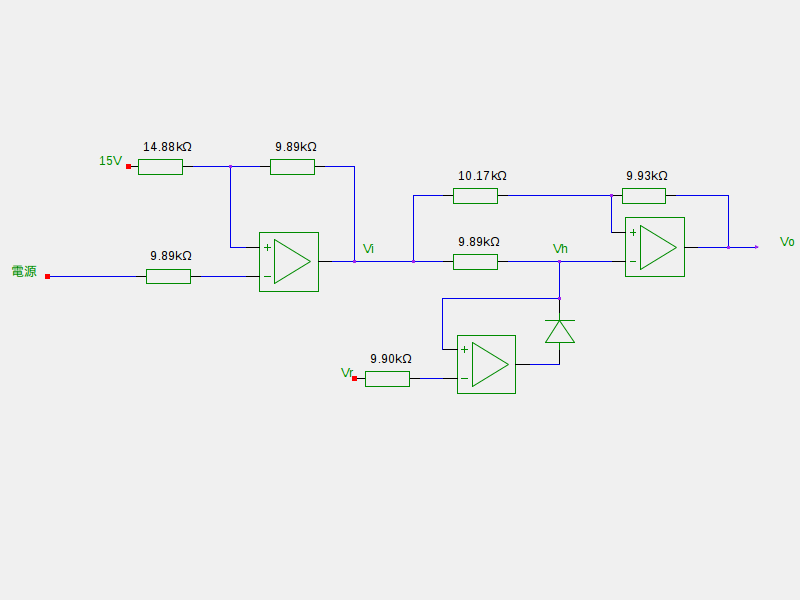
\includegraphics[width=8cm,clip]{abs_tokusei.png}
  \caption{絶対値回路の測定回路}
  \label{fig:abs_tokusei}
 \end{figure}%
    
    \begin{figure}[htbp]
  \centering
  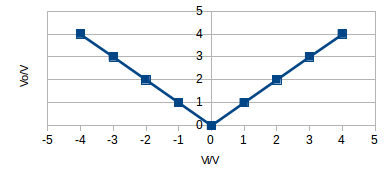
\includegraphics[width=8cm,clip]{risou_absr0.png}
  \caption{基準電圧0Vの時の理想的な絶対値回路の原理グラフ}
  \label{fig:risou_absr0}
 \end{figure}
    
    \begin{figure}[htbp]
  \centering
  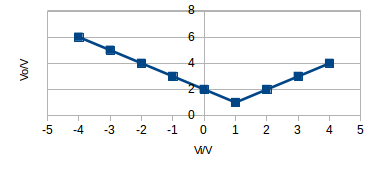
\includegraphics[width=8cm,clip]{risou_absr1.png}
  \caption{基準電圧1Vの時の理想的な絶対値回路の原理グラフ}
  \label{fig:risou_absr1}
 \end{figure}
    
    
    
   \subsubsection{測定手順}
    絶対値回路について、直流電源に対して全波整流の挙動を測定。
    \begin{enumerate}
    \item 図\ref{fig:abs_tokusei}の回路を設計。
    \item 基準電圧$V_r$、入力電圧$V_i$を変動させ出力電圧$V_o$の挙動を測定。
    \end{enumerate}
    
   \subsubsection{結果と考察} \label{sec:abs_tokusei}
    
    図\ref{fig:2_Vr0}、\ref{fig:2_Vr1}にはそれぞれ基準電圧が0Vと1Vのときの絶対値回路の直流電源に対する入出力特性データを示す。
    
    \begin{figure}[htbp]
  \centering
  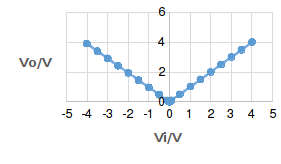
\includegraphics[width=8cm,clip]{2_Vr0.png}
  \caption{基準電圧$V_r$=0Vの時の絶対値回路の入出力特性}
  \label{fig:2_Vr0}
 \end{figure}%
    
    \begin{figure}[htbp]
  \centering
  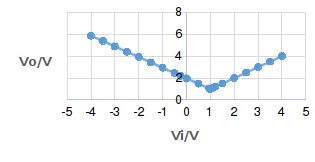
\includegraphics[width=8cm,clip]{2_Vr1.png}
  \caption{基準電圧$V_r$=1Vの時の絶対値回路の入出力特性}
  \label{fig:2_Vr1}
 \end{figure}%
    
    上記のように基準電圧を変動させることにより出力特性を変化させることができる。ただしこのデータからそのグラフの形が変化するのではなく、原点のみが移動している、ということがわかりその入出力関係は
    \begin{eqnarray}
    V_o &=& V_i (V_i > 1) \\
           &=& - V_i + 2 (V_i <1)
    \end{eqnarray}
    という式で表される。実際この式は理想的な絶対値回路についてと同様で成り立つことである。
        
    
    
  \subsection{絶対値回路の入出力波形測定}
   \subsubsection{原理}
    
    図\ref{fig:abs_wave}に絶対値回路の波形観測回路を示す。
    
    \begin{figure}[htbp]
  \centering
  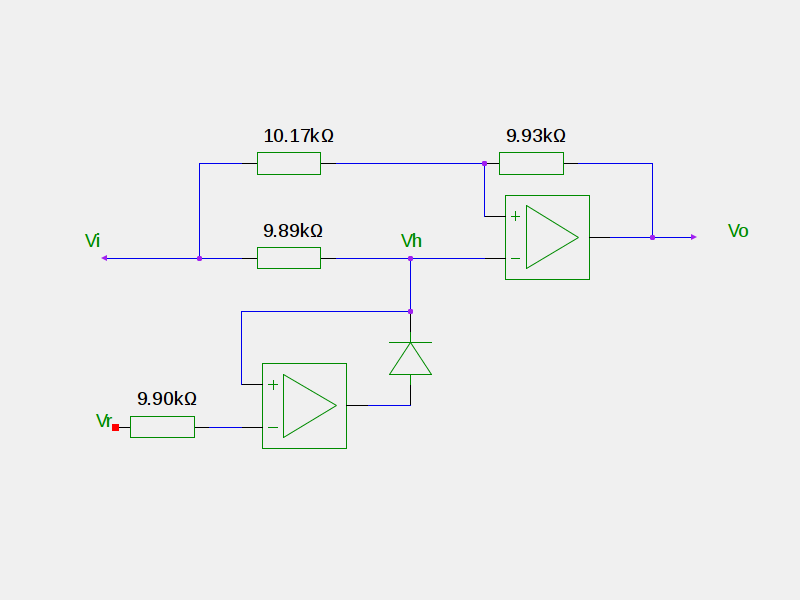
\includegraphics[width=8cm,clip]{abs_wave.png}
  \caption{絶対値回路の波形観測回路}
  \label{fig:abs_wave}
 \end{figure}%
    
   \subsubsection{測定手順}
    絶対値回路について、交流電源に対する全波整流作用を観測。
    \begin{enumerate}
    \item 図\ref{fig:abs_wave}の回路を設計。
    \item 基準電圧$V_r$、入力周波数、振幅、波形(ex.正弦波、三角波)による出力の変動を測定。
    \end{enumerate}
    
   \subsubsection{結果と考察} \label{sec:abs_wave}
    
    図\ref{fig:2_Vr0_sin}~\ref{fig:2_Vr1_4}に基準電圧と振幅、波形によりそれぞれ場合分けして観測した波形データを示す。
    
    このデータを見てみると、その全てで基準電圧を基準として整流作用が表れていることがわかる。図\ref{fig:2_Vr1_4}などには半値整流が内容に見えるが、これはその出力の全範囲が基準電圧以上であるため入力がそのまま出力されていることになる。ただし図\ref{fig:2_Vr0_sin}などの高周波数では遅延が確認できる。これは前述のリミッタについてと同様で、ダイオードの空乏層容量によるコンデンサーとしての振る舞いが原因だと考えられる。
    
    またこの絶対値回路を全波整流とみなしたときの平均電圧の計算、及び気宇順電圧を1Vとした場合の出力電圧の平均値の計算を付録として掲載する。
    
    \begin{figure}[htbp]
  \centering
  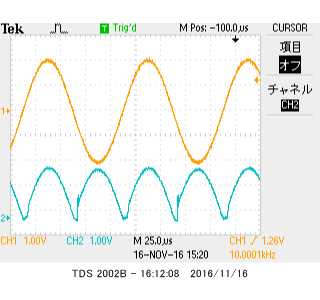
\includegraphics[width=8cm,clip]{2_abs_Vr0_f10V4sin_ViVo.png}
  \caption{基準電圧なしの絶対値回路の波形(f=10kHz,Vpp=4V,正弦波)}
  \label{fig:2_Vr0_sin}
 \end{figure}%
    
    
    \begin{figure}[htbp]
  \centering
  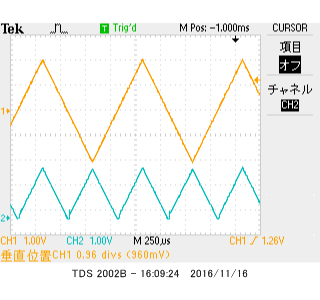
\includegraphics[width=8cm,clip]{2_abs_Vr0_f1V4sankaku_ViVo.png}
  \caption{基準電圧なしの絶対値回路の波形(f=1kHz,Vpp=4V,三角波)}
  \label{fig:2_Vr0_sankaku}
 \end{figure}%
  
  \begin{figure}[htbp]
  \centering
  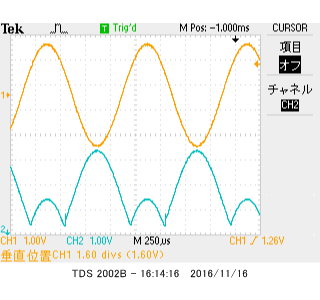
\includegraphics[width=8cm,clip]{2_abs_Vr1_f1V2sin_ViVo.png}
  \caption{基準電圧1Vの絶対値回路の波形(f=1kHz,Vpp=2V)}
  \label{fig:2_Vr1_2}
 \end{figure}%
  
  
  \begin{figure}[htbp]
  \centering
  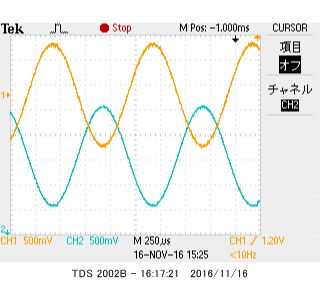
\includegraphics[width=8cm,clip]{2_abs_Vr1_f1V4sin_ViVo.png}
  \caption{基準電圧1Vの絶対値回路の波形(f=1kHz,Vpp=4V)}
  \label{fig:2_Vr1_4}
 \end{figure}%
  
  
  \clearpage
  
  %レポート課題
 \section{レポート課題} 
  \begin{itemize}
  \item a)レベルシフタの\ref{sec:le_kousatu}結果と考察、を参照。
  \item b)\ref{sec:noamp_tokusei}の「オペアンプなしリミッタの入出力特性」、及び\ref{sec:amp_tokusei}の「オペアンプありリミッタの入出力特性」の「実験と考察」の項を参照。
  \item c)\ref{sec:noamp_wave}の「オペアンプなしリミッタの入出力波形観測」の「実験と考察」の項を参照。
  \item d)\ref{sec:amp_wave}の「オペアンプありリミッタの入出力波形観測」の「実験と考察」の項を参照。
  \item e)\ref{sec:noamp_wave}の「オペアンプなしリミッタの入出力波形観測」の「実験と考察」の項、\ref{sec:amp_wave}の「オペアンプありリミッタの入出力波形観測」の「実験と考察」の項、及び付録を参照。
  \item f)\ref{sec:histeri}の「ヒステリシスコンパレータの入出力波形観測」の「実験と考察」の項を参照。
  \item g)\ref{sec:histeri}の「ヒステリシスコンパレータの入出力波形観測」の「実験と考察」の項を参照。
  \item h)\ref{sec:abs_tokusei}の「絶対値回路の入出力特性」の「実験と考察」の項を参照。
  \item i)\ref{sec:abs_wave}の「絶対値回路の波形観測」の「実験と考察」の項を参照。
  \item j)\ref{sec:abs_wave}の「絶対値回路の波形観測」の「実験と考察」の項、及び付録を参照。
  \item k)\ref{sec:abs_wave}の「絶対値回路の波形観測」の「実験と考察」の項、及び付録を参照。
  \end{itemize}
  
  %まとめ
  \section{まとめ}
  今回の実験ではアナログ回路を用いた非線形計算の実現を学習してきた。この非線形計算は単純な電卓のような計算として利用されることはなく、様々な物理的な測定、センサー、及びスイッチとして利用される。
  
  リミッタによる半波整流、ヒステリシスコンパレータによるノイズ除去、絶対値回路による全波整流を物理的なシステムに応用することが本実験を通して学んだエッセンスであり、次期の目的である。
  
  %参考文献
 \section{参考文献}
  [1]雨宮好文、「現代電子回路学」、オーム社
  
  [2]古川静二郎、「電子デバイス工学・第2版」、森北出版株式会社、p.45~50
  
  
\end{document}